\documentclass[conference]{IEEEtran}

\usepackage{cite}
\usepackage{amsmath,amssymb}
\usepackage{graphicx}
\usepackage{hyperref}

\begin{document}

\title{AI-Assisted Programming in Software Engineering: A Systematic Literature Review and Socio-Technical Perspective}

\author{
\IEEEauthorblockN{L.F. Guevara-Chávez}
\IEEEauthorblockA{
School of Engineering and Science \\
Tecnológico de Monterrey \\
Tampico, México \\
leon.guevara@tec.mx}
}

\maketitle

\begin{abstract}
The rapid adoption of AI-assisted programming tools, particularly those based on large language models (LLMs), has significantly transformed software development practices. While these tools promise substantial productivity gains, existing evidence remains fragmented and, in some cases, contradictory. This study presents a systematic literature review of empirical research published between 2021 and 2026, synthesising findings from controlled experiments, large-scale observational studies, industrial deployments, and qualitative investigations.

The analysis integrates evidence across multiple dimensions, including productivity, code quality, technical debt, human--AI interaction, cognitive load, organisational impact, economic viability, and developer perception. Results indicate that AI-assisted programming consistently increases development output; however, these gains are often accompanied by trade-offs, such as higher verification effort, increased technical debt, and shifts in maintenance responsibilities. Furthermore, the effectiveness of these tools is highly contingent on factors such as developer experience, intensity of adoption, and the quality of human--AI interaction, particularly in iterative prompting and validation processes.

The findings also reveal a notable gap between perceived and actual productivity, as well as the importance of cognitive and sociotechnical factors, including trust calibration and community-driven heuristics, in shaping tool usage. From an economic perspective, AI-assisted development can be viable under appropriate conditions, although it introduces additional costs related to training, supervision, and integration.

Overall, this study advances a socio-technical equilibrium perspective of AI-assisted programming, arguing that its value emerges not from linear automation, but from the managed balance between generation efficiency, verification effort, interaction quality, trust calibration, and organisational context.
\end{abstract}

\section{Introduction}

\subsection{Background}

The emergence of AI-assisted programming tools, particularly those powered by large language models (LLMs), has introduced a significant shift in software development practices. Tools such as GitHub Copilot and conversational AI systems are increasingly integrated into development workflows, enabling developers to generate code, debug, and explore solutions through natural language interaction \cite{cui_productivity_2024, rasnayaka_empirical_2024}.

Early evidence suggests that these tools can accelerate software development by reducing the time required to produce code and by automating repetitive tasks \cite{kumar_intuition_2025}. However, the benefits of AI-assisted programming are not uniformly distributed and appear to depend on factors such as developer experience, task complexity, and the level of tool adoption \cite{xu_ai-assisted_2026, koripalli_copilot_2025}.

At the same time, concerns have been raised regarding the quality and reliability of AI-generated code. Empirical studies have reported increased defect rates, higher levels of technical debt, and the persistence of errors across iterative interactions with AI systems \cite{sandoval_lost_2022, zhong_developer-llm_2025}. These findings suggest that improvements in productivity may be accompanied by hidden costs, particularly in verification and maintenance activities.

Beyond technical outcomes, AI-assisted programming fundamentally changes how developers interact with software systems. Rather than acting as passive tools, AI systems participate in iterative, multi-turn interactions that require active prompting, validation, and refinement by the user \cite{zhong_developer-llm_2025, pinto_developer_2024}. This shift introduces new cognitive and behavioral dynamics, including changes in problem-solving strategies and reliance on AI-generated suggestions.

Recent research has also highlighted the role of human factors in mediating the effectiveness of AI-assisted development. Studies on cognitive load indicate that AI tools can reduce perceived effort and improve task performance under certain conditions \cite{brachten_ability_2020}. However, these benefits depend on the user's ability to effectively interact with the system, including prompt formulation and error identification.

From an organisational perspective, the adoption of AI-assisted programming tools has been associated with changes in team dynamics and workflows. Evidence suggests a redistribution of effort, where less experienced developers increase their output while more experienced developers spend more time reviewing and validating code \cite{koripalli_copilot_2025}. This redistribution raises important questions about long-term sustainability and skill development.

In addition, economic analyses indicate that AI-assisted programming can be financially viable, offering a positive return on investment under appropriate conditions. However, these benefits must be weighed against additional costs related to training, supervision, and integration into existing workflows \cite{rodriguez_comparative_nodate}.

Finally, studies based on user perception reveal a gap between perceived and actual productivity gains. While developers often report positive experiences with AI tools, a significant portion of their time may still be spent verifying and correcting AI-generated outputs \cite{lyu_my_2025}. This discrepancy underscores the importance of distinguishing between subjective experience and objective performance.

Despite the growing number of empirical studies, there remains a lack of integrative frameworks that explain how these effects interact across technical, human, and organisational dimensions. This study addresses this gap by providing a unified, multidimensional synthesis of AI-assisted programming.

\subsection{Problem Statement}

Despite the growing body of research, the impact of AI-assisted programming remains fragmented across multiple dimensions, including productivity, code quality, human--AI interaction, cognitive load, and economic outcomes. Existing studies often focus on isolated aspects, making it difficult to form a coherent understanding of how these tools affect software development as a whole.

Moreover, the literature presents conflicting findings. While some studies report substantial productivity gains, others highlight increased verification effort, technical debt, and maintenance overhead. Similarly, user perception studies often diverge from empirical measurements, revealing inconsistencies between how developers experience AI tools and how these tools actually affect performance.

\subsection{Research Objective}

The goal of this study is to systematically synthesise empirical evidence on AI-assisted programming in software engineering, integrating findings across technical, human, and organisational dimensions.

\subsection{Research Question}

RQ1: What is the impact of AI-assisted programming on software development processes and outcomes?

\subsection{Contributions}

This study makes the following contributions:

\begin{itemize}
    \item A systematic synthesis of 128 empirical studies on AI-assisted programming across seven analytical dimensions.
    \item Evidence of a systematic trade-off between productivity gains, verification effort, code quality, and socio-technical complexity.
    \item A socio-technical equilibrium perspective that explains contradictory findings in the literature.
    \item Identification of prompting and validation literacy as emerging professional competencies in AI-assisted software development.
\end{itemize}

\section{Methodology}

\subsection{Research Design}

This study follows a Systematic Literature Review (SLR) methodology, structured according to established evidence-based software engineering guidelines \cite{kitchenham2007guidelines} and the PRISMA framework \cite{page2021prisma} to ensure transparency, rigour, and reproducibility.

The objective is to identify, evaluate, and synthesise empirical evidence regarding the impact of AI-assisted programming tools on software development. The review process was designed as a multi-stage protocol including search, screening, eligibility assessment, quality evaluation, and synthesis.

In addition to primary empirical studies retrieved through the main search process, a limited number of foundational and related works published outside the main search window were retained to support conceptual framing, historical grounding, and interpretation. These works were not counted as part of the main empirical evidence base.

\subsection{Research Question}

The study is guided by the following research question:

\begin{itemize}
    \item RQ1: What is the impact of AI-assisted programming on software development processes and outcomes?
\end{itemize}

To address this question, the analysis was structured across seven analytical dimensions: productivity, code quality and technical debt, human--AI interaction, cognitive load, organisational impact, economic impact, and perception and trust.

\subsection{Search Strategy}

The search process combined AI-assisted literature discovery with manual screening and validation, using both academic databases and complementary discovery tools. An initial broad search was conducted using SciSpace as an academic discovery assistant, supported by complementary searches in major academic databases.

A structured search instruction was provided to SciSpace to retrieve studies related to AI-assisted programming and LLM-based code generation tools, including GitHub Copilot, ChatGPT, Amazon CodeWhisperer, Claude Code, Gemini, and OpenAI Codex. The instruction incorporated the review topic, research questions, time window, inclusion and exclusion criteria, output requirements, and quality control constraints.

The literature search was conducted using the following academic databases:
\begin{itemize}
    \item arXiv
    \item ACM Digital Library
    \item IEEE Xplore
    \item SpringerLink
    \item Elsevier (ScienceDirect)
    \item ProQuest
\end{itemize}

The search targeted publications between 2021 and 2026, reflecting the emergence and rapid evolution of modern AI-assisted coding tools. The search strategy prioritised empirical studies reporting measurable outcomes related to software development.

Rather than relying on a single keyword string, the initial retrieval process was guided by a structured semantic query protocol implemented through SciSpace. This approach was used to capture a broad and verifiable set of candidate studies aligned with the review scope. The full search instruction can be provided as supplementary material.

\subsection{Use of Artificial Intelligence in the Review Process}

Artificial intelligence tools were used to support parts of the literature review process, particularly for:
\begin{itemize}
    \item Initial literature discovery and retrieval through SciSpace
    \item Relevance-based screening suggestions
    \item Extraction and structuring of metadata
\end{itemize}

During the initial search stage, SciSpace was used as an academic discovery assistant to support literature discovery and retrieval. Its operation was guided by a structured instruction that specified the review topic, research questions, inclusion and exclusion criteria, publication window, and required output fields.

However, all critical decisions regarding inclusion, exclusion, classification, quality assessment, and synthesis were performed and validated manually by the author. AI outputs were treated strictly as assistive recommendations rather than as final selection decisions.

\subsection{Inclusion and Exclusion Criteria}

Studies were included if they met the following criteria:
\begin{itemize}
    \item Empirical evaluation (quantitative, qualitative, or mixed-methods)
    \item Focus on AI-assisted programming or code generation
    \item Evaluation of modern AI tools (e.g., Copilot, ChatGPT, Codex, Gemini)
    \item Reporting of empirical results, evaluation metrics, or qualitative findings that allow analytical interpretation
    \item Published between 2021 and 2026
    \item Written in English
\end{itemize}

Studies were excluded if they:
\begin{itemize}
    \item Were opinion papers, editorials, or non-scientific content
    \item Lacked empirical or analytical grounding
    \item Focused on unrelated NLP tasks
    \item Were duplicate or overlapping versions of the same study
\end{itemize}

To improve dataset consistency, weak or redundant studies were excluded during early screening stages rather than during final selection, resulting in a more coherent and analytically robust dataset.

\subsection{Study Selection Process}

The review process followed PRISMA 2020 guidelines \cite{page2021prisma} to ensure transparency and reproducibility. The study selection process consisted of four phases:

\begin{enumerate}
    \item Identification: Initial retrieval of a broad set of candidate studies through SciSpace and complementary academic database searches
    \item Screening: Removal of duplicate and irrelevant records based on title and abstract evaluation
    \item Eligibility: Full-text assessment to ensure empirical relevance and methodological adequacy
    \item Inclusion: Final selection of studies for synthesis and analysis
\end{enumerate}

The initial AI-assisted retrieval stage produced 1,255 records. After removal of duplicates, 863 records remained for screening. Title and abstract evaluation excluded 508 records, and 355 studies proceeded to full-text assessment. After full-text screening, 349 studies were retained in the broader qualitative synthesis set.

The screening process was conducted manually by the author using a structured and consistently applied evaluation protocol. To improve dataset consistency, weak, redundant, or analytically peripheral studies were excluded during the refinement stages.

From this broader set, a final dataset of 128 empirical studies was selected for the core analytical synthesis reported in this paper. In addition, a smaller number of foundational and related works were retained to support conceptual framing and interpretation, but were not counted as part of the main empirical evidence base.

To reduce potential bias, the selection and classification process was applied consistently through multiple validation passes following a structured evaluation protocol.

\subsection{Quality Assessment}

A multi-criteria evaluation framework was used to assess study quality, considering:

\begin{itemize}
    \item Empirical rigour (e.g., experimental design, sample size)
    \item Methodological strength (e.g., causal inference vs. observational)
    \item Venue quality
    \item Completeness and transparency of reporting
    \item Relevance to the research question
\end{itemize}

This framework was applied consistently across all studies to ensure comparability and reduce subjective bias in quality assessment. The assessment was conducted manually to ensure careful evaluation of study design and reporting quality.

Studies were classified into three categories:

\begin{itemize}
    \item A1: High rigour (e.g., controlled experiments, large-scale empirical or causal studies)
    \item A2: Moderate rigour (e.g., user studies, case studies, structured evaluations)
    \item B: Supporting evidence (e.g., perception studies, qualitative analyses, or model-based approaches)
\end{itemize}

This classification was used to prioritise higher-quality studies (A1 and A2) in the synthesis and interpretation of results, ensuring that the main conclusions are grounded in the most robust evidence, while category B studies were primarily used to provide contextual support and complementary insights.

\subsection{Data Extraction and Synthesis}

Data extraction was performed by systematically reviewing each selected study and recording key attributes using a structured extraction template to ensure consistency across studies.

For each study, the following data were extracted:

\begin{itemize}
    \item Study type and methodological classification
    \item Tools evaluated
    \item Evaluation metrics
    \item Key findings
    \item Associated analytical dimensions
\end{itemize}

Given the heterogeneity of study designs, metrics, and evaluation contexts, a formal meta-analysis was not feasible. Instead, a structured synthesis approach was adopted to identify consistent patterns and trends across studies. This approach is consistent with established practices in systematic literature reviews, where high variability limits the applicability of statistical meta-analysis.

The reported percentages were derived from structured coding of the selected studies based on titles, abstracts, and available metadata, following a consistent categorisation scheme to identify broad trends in the literature.

The analysis combined quantitative aggregation (e.g., frequency distributions) with qualitative synthesis to identify patterns, contradictions, and research gaps across dimensions.

\subsection{PRISMA Study Selection}

\begin{table}[h]
\centering
\caption{PRISMA 2020 Screening Summary}
\label{tab:prisma_summary}
\begin{tabular}{l r}
\hline
\textbf{Stage} & \textbf{Records ($n$)} \\
\hline
Identified (SciSpace + Google Scholar) & 1,255 \\
Duplicates removed & 392 \\
After deduplication & 863 \\
Excluded at abstract screening & 508 \\
\quad Lack of empirical validation & (215) \\
\quad Non-programming NLP tasks & (178) \\
\quad Inaccessible research context & (115) \\
Proceeding to full-text assessment & 355 \\
Excluded at full-text screening & 6 \\
\quad Insufficient methodological detail & (3) \\
\quad Lack of AI code generation focus & (2) \\
\quad Inaccessible research context & (1) \\
\textbf{Included in qualitative synthesis} & \textbf{349} \\
\textbf{Core empirical dataset used for main analysis} & \textbf{128} \\
\hline
\end{tabular}
\end{table}

The PRISMA counts reported in Table~\ref{tab:prisma_summary} reflect the broad retrieval and screening phase of the review. From the 349 studies retained in the qualitative synthesis pool, an additional quality-based and analytical refinement process was applied to construct the final core dataset of 128 empirical studies used in the main results of this paper, as shown in Fig.~\ref{fig:prisma_diagram}. The refinement from 349 studies to the final core dataset of 128 studies was based on methodological quality, direct relevance to the seven analytical dimensions, empirical depth, and the removal of studies with overlapping or peripheral contributions. Foundational and related works were retained separately for conceptual framing and contextual support.

\begin{figure}[h]
    \centering
    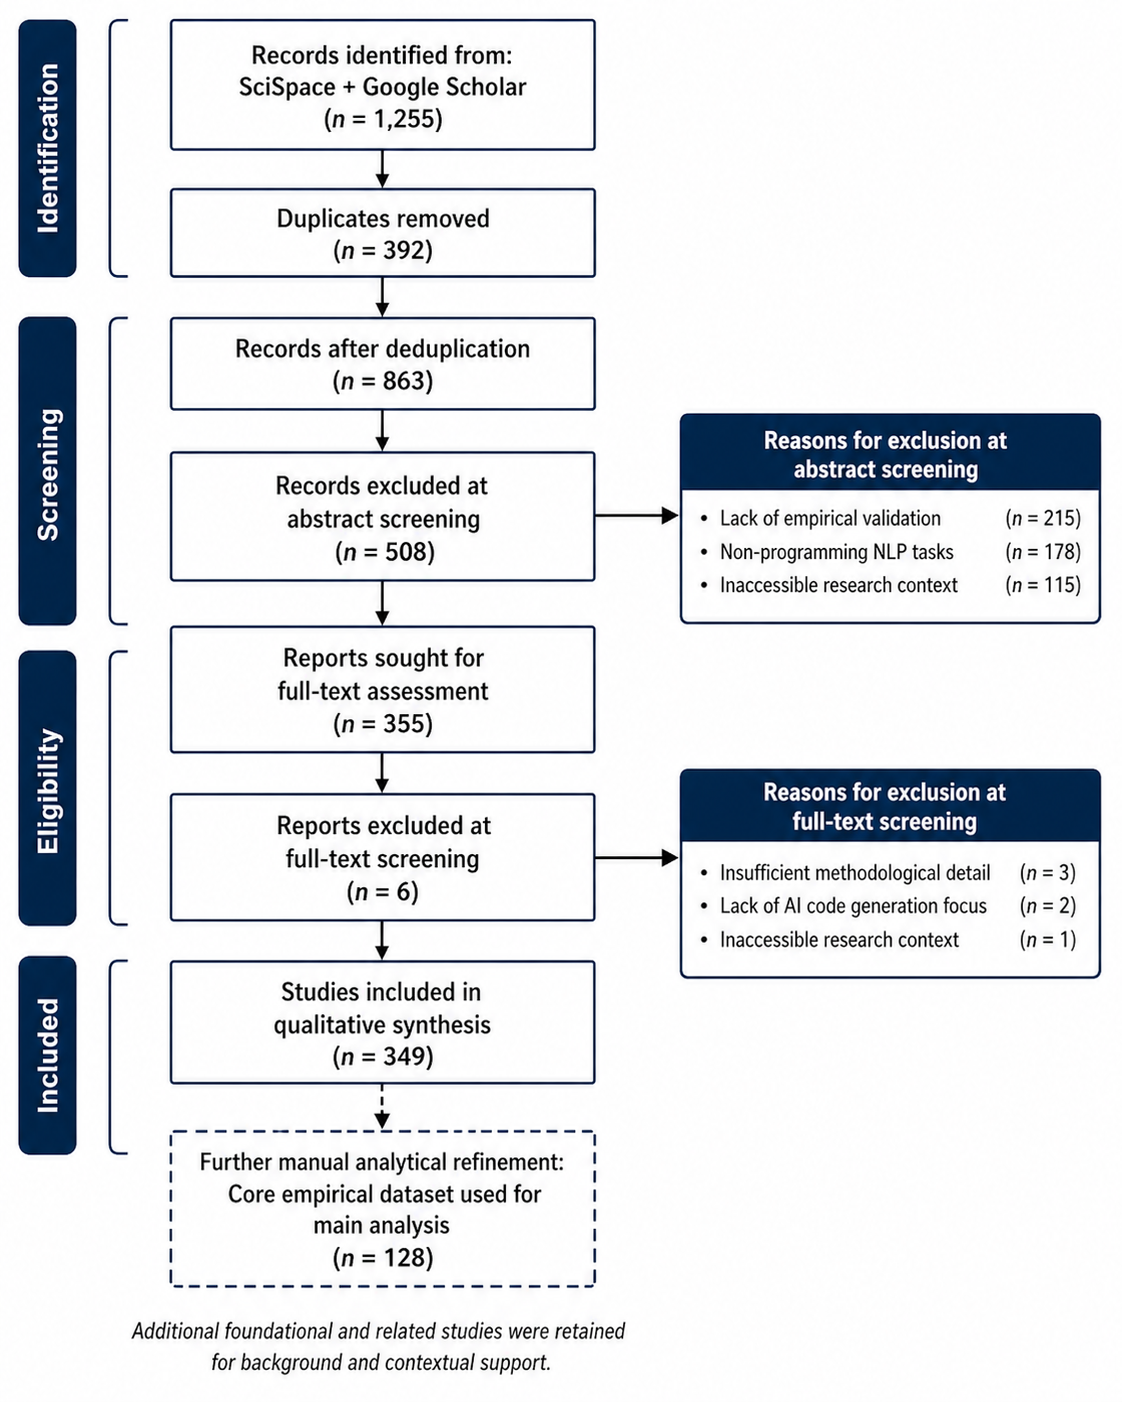
\includegraphics[width=0.9\linewidth]{figures/prisma_diagram.png}
    \caption{PRISMA 2020 Study Selection Diagram}
    \label{fig:prisma_diagram}
\end{figure}


A quantitative meta-analysis was not conducted due to the heterogeneity of study designs, evaluation metrics, and experimental contexts, which limited direct comparability across studies.

\section{Results}

\subsection{Corpus Profile and Evidence Hierarchy}

The final dataset comprises 128 studies, reflecting a heterogeneous body of evidence in terms of methodological rigour, evaluation context, and analytical focus. Studies were classified into three categories: A1 (high rigour), A2 (moderate rigour), and B (supporting or qualitative evidence).

Out of the 128 studies, 39.8\% were classified as A1, 51.6\% as A2, and 8.6\% as B, as shown in Fig.~\ref{fig:main_classification}. This distribution indicates that the majority of the evidence base is grounded in empirical studies with moderate-to-high methodological rigour.

\begin{figure}[h]
    \centering
    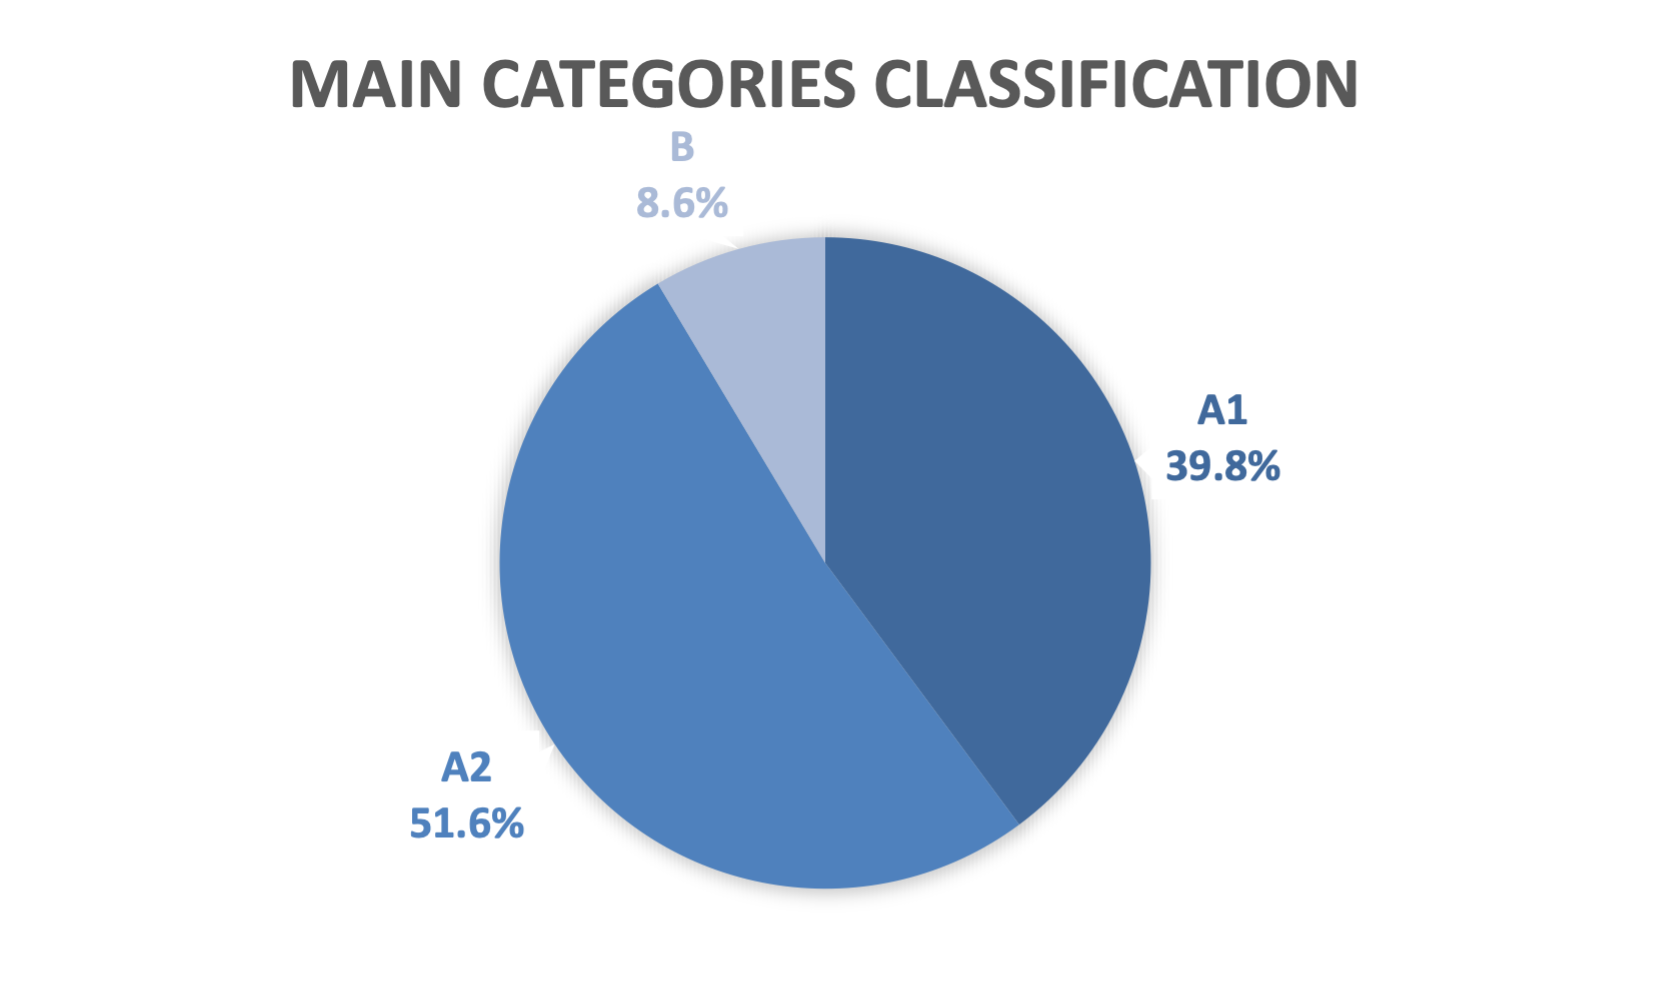
\includegraphics[width=0.82\linewidth]{figures/main_classification.png}
    \caption{Distribution of the final dataset by evidence class (A1, A2, and B).}
    \label{fig:main_classification}
\end{figure}

In terms of analytical dimensions, as shown in Fig.~\ref{fig:dimensions}, the largest proportion of studies focused on productivity (29.7\%) and code quality and technical debt (27.3\%), followed by human--AI interaction (15.6\%) and perception and trust (10.2\%). Fewer studies addressed economic impact (9.4\%), organisational aspects (5.5\%), and cognitive load (2.3\%).

\begin{figure}[h]
    \centering
    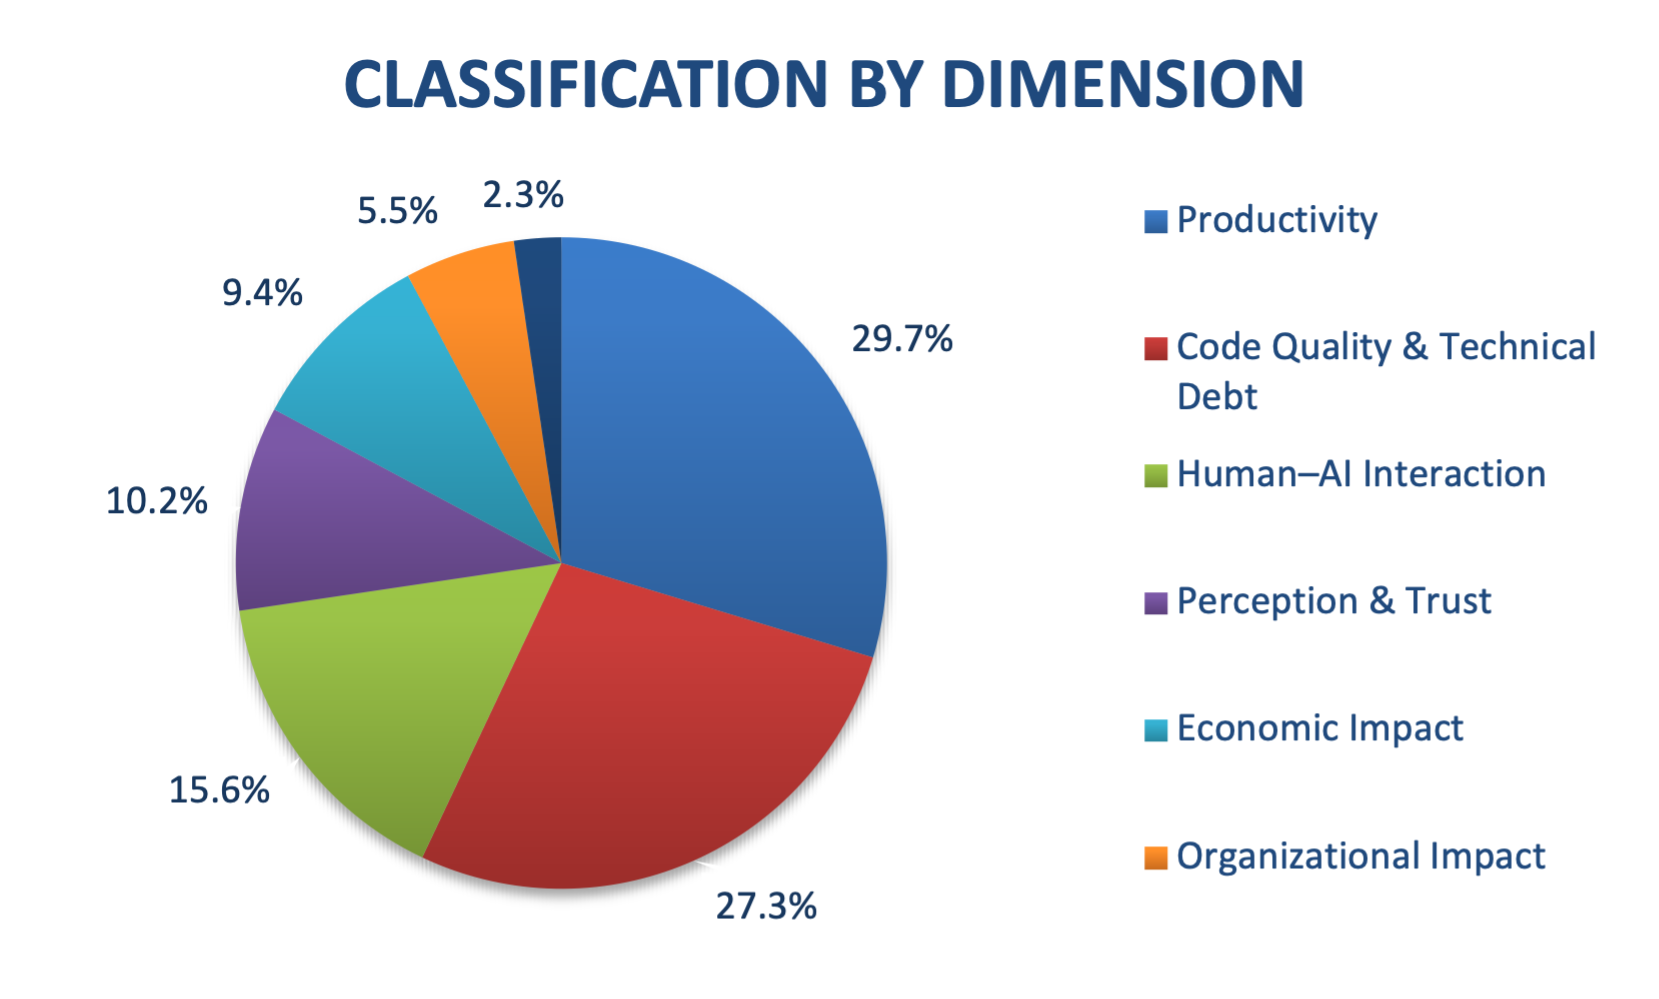
\includegraphics[width=0.82\linewidth]{figures/dimensions.png}
    \caption{Distribution of included studies across the seven analytical dimensions.}
    \label{fig:dimensions}
\end{figure}

High-rigour studies include controlled experiments, large-scale observational analyses, and quasi-experimental designs \cite{cui_productivity_2024, xu_ai-assisted_2026, kumar_intuition_2025}, while A2 studies include structured user evaluations and contextual analyses \cite{rasnayaka_empirical_2024, koripalli_copilot_2025}. Supporting studies (B) provide qualitative insights, perception-based evidence, and model-driven analyses \cite{lyu_my_2025}.

This classification enables a weighted synthesis, where conclusions are primarily grounded in stronger empirical evidence. It also reveals a clear concentration of research efforts on technical performance outcomes, with comparatively limited attention to cognitive, organisational, and economic dimensions.

\subsection{Productivity Effects: Gains Under Conditional Contexts}

Productivity is the most extensively studied dimension, accounting for approximately 29.7\% of the analysed literature. Across the corpus, there is consistent evidence that AI-assisted programming improves developer productivity, particularly in terms of task completion speed and code generation. This pattern is further supported by quantitative evidence: productivity gains in routine and well-defined tasks typically range between 30\% and 55\%, while improvements in more complex and realistic development scenarios tend to fall between 27\% and 47\%. In some cases, task completion time reductions of up to 46.4\% have been reported in repetitive workflows. High-rigour studies report measurable gains in routine and well-defined tasks, such as boilerplate code generation, API integration, and initial debugging \cite{cui_productivity_2024, xu_ai-assisted_2026, kumar_intuition_2025}. These improvements are especially pronounced for less experienced developers and in early-stage development activities.

These productivity gains are not uniform across task types. Evidence shows that AI-assisted programming is particularly effective in routine and repetitive activities, such as code documentation, boilerplate generation, and unit testing. In industrial settings, time savings of up to 50\% have been reported for documentation and autocompletion tasks, and between 30\% and 40\% for repetitive development activities \cite{pandey_transforming_nodate}. Correcting almost correct AI-generated code can save from 8.9\% to 71.3\% of time when compared to programming from scratch \cite{idrisov_program_2024}.

Similarly, enterprise studies report productivity improvements of up to 55\% in routine implementation tasks, while gains in complex activities such as architectural design and algorithm development are substantially lower, typically ranging between 8\% and 12\%. This gap highlights a fundamental limitation: AI-assisted programming performs well in localised, well-defined contexts but struggles to maintain effectiveness in tasks requiring system-level reasoning \cite{koripalli_copilot_2025}.

However, these gains are conditional. Evidence indicates that productivity improvements diminish as task complexity increases, particularly in scenarios involving architectural decisions, multi-module integration, or domain-specific logic \cite{rasnayaka_empirical_2024, koripalli_copilot_2025}. In such cases, the need for validation, correction, and iterative refinement offsets part of the initial efficiency gains.

The effectiveness of AI-generated code also declines significantly when external dependencies or cross-module interactions are involved. In such cases, success rates can drop, ranging between 4\% and 16\%, indicating limited capability to handle broader system context \cite{corso_generating_2024}.

This discrepancy is further reflected in the difference between controlled and real-world scenarios. While programming, ``puzzle'' tasks can be completed up to 55.8\% faster with AI assistance, these gains are substantially reduced or absent in realistic software development tasks that require deeper conceptual understanding of the system \cite{xu_ai-assisted_2026, wang_rocks_2024}.

Taken together, these results show a clear pattern: performance gains decrease systematically as task complexity increases.

The impact of AI-assisted programming varies significantly with developer experience. Less experienced developers tend to exhibit larger relative productivity gains, with some large-scale deployments reporting increases of up to 77\% in code contributions for junior developers, compared to approximately 45\% for mid-level and senior developers \cite{kumar_intuition_2025}.

AI-assisted programming reduces barriers to contribution, enabling peripheral contributors to increase their activity by up to 43.5\% in mature codebases. However, these gains come with important caveats. Some studies report a decrease of up to 28\% in algorithmic problem-solving ability among less experienced developers after prolonged reliance on AI tools, suggesting potential negative effects on skill development \cite{xu_ai-assisted_2026, koripalli_copilot_2025}.

Taken together, these results indicate that productivity gains are inherently conditional, varying systematically with task complexity, developer expertise, and interaction dynamics.

Manual review of AI-generated code is often time-consuming and cognitively demanding, partially offsetting initial productivity gains. In team settings, this effect is amplified: while less experienced developers produce more code, experienced developers may experience a decrease in their own coding productivity (up to 19\%) due to increased time spent reviewing and reworking AI-generated contributions \cite{xu_ai-assisted_2026}.

This dynamic introduces a gap between code quantity and code quality. Although more lines of code are produced, this code is often subject to higher rates of modification and deletion in later stages, indicating increased rework and potential technical debt \cite{imai_is_2022}.

In this sense, AI-assisted programming increases output more reliably than it improves overall development efficiency.

Within the emerging socio-technical structure, these findings reflect a redistribution of effort from code generation toward validation and decision-making activities.

\subsection{Code Quality and Technical Debt}

Code quality and technical debt represent 27.3\% of the corpus and constitute the second most extensively studied dimension. While AI-assisted tools are capable of producing syntactically correct code, multiple studies report increased risks of defects, vulnerabilities, and maintainability issues. Quantitative analyses indicate that a substantial portion of AI-generated code falls into the category of "correct but vulnerable", with reported rates ranging from approximately 34\% to 44\%. Additionally, incorrect outputs can range from 12\% to over 50\% depending on the model and task complexity, highlighting significant reliability concerns. These ranges vary depending on model, dataset, and evaluation context, but consistently indicate substantial variability in reliability.

In many cases, AI-generated code is syntactically correct but semantically shallow. Generated solutions often rely on simplified logic, reduced lexical diversity, and underdeveloped class structures, which may overlook edge cases and deeper system requirements \cite{cotroneo_human-written_2025}.

Empirical analyses show that a large proportion of detected issues correspond to maintainability concerns rather than functional failures. In some studies, between 90\% and 93\% of identified issues in AI-generated code are classified as code smells, indicating degraded maintainability and increased long-term costs \cite{sabra_assessing_2025}.

Evidence indicates that AI-generated code can introduce subtle logical errors and inconsistencies, particularly in security-sensitive contexts where incorrect assumptions or incomplete implementations may lead to exploitable vulnerabilities \cite{sandoval_lost_2022}. Overall, these findings consistently indicate that reliability issues are not isolated, but systemic across models and contexts.

Beyond general defects, multiple studies report the systematic introduction of security vulnerabilities in AI-generated code. Common issues include command injection (CWE-78), hardcoded credentials (CWE-259), and SQL injection (CWE-89), which appear consistently across multiple models and programming languages \cite{schreiber_security_2026}.

Comparative analyses further indicate that AI-generated code may be more vulnerable than human-written code \cite{cotroneo_human-written_2025}. Large-scale studies report that AI-generated code contains, on average, up to 6.4\% more security vulnerabilities than code written by developers \cite{kim_security_2025}. Additionally, AI systems often fail to reliably detect vulnerabilities in their own outputs, exhibiting high rates of false positives and blind spots during self-evaluation \cite{gong_how_2025}.

Additionally, large-scale interaction studies show that errors can propagate across multi-turn interactions, where initial inaccuracies—such as undefined variables or incorrect assumptions—persist or even intensify as developers iteratively refine the code \cite{zhong_developer-llm_2025}.

In addition, studies report a higher incidence of simple but persistent bugs, such as single-statement errors, which can occur at significantly higher rates than in correct code. These issues often require disproportionate effort to identify and correct, further contributing to technical debt \cite{jesse_large_2023}.

Quasi-experimental evidence further suggests that increased output volume may result in higher rework rates, as developers must revisit and correct AI-generated code \cite{xu_ai-assisted_2026}. Collectively, these findings highlight a structural tension between speed and reliability, where gains in productivity may come at the cost of long-term code quality. This suggests that improvements in code generation capability do not necessarily translate into improvements in code correctness or robustness.

In practice, AI-generated code is rarely integrated without modification. Developers frequently report the need for substantial revision to ensure compatibility, correctness, and security \cite{siddiq_quality_2024}.

This effect is compounded by overconfidence, particularly among less-experienced developers, who may incorrectly assess insecure or incomplete code as correct because of its apparent plausibility. As a result, AI-assisted programming can increase the risk of latent defects being introduced into production systems \cite{perry_users_2023}.

Taken together, these findings highlight a structural trade-off between generation efficiency and long-term code reliability.

\subsection{Human--AI Interaction and Prompting Dynamics}

The limitations observed in code quality and reliability are closely linked to the interaction dynamics between developers and AI systems.

Human--AI interaction accounts for 15.6\% of the analysed studies and emerges as a key explanatory factor for performance variability. AI-assisted programming is inherently interactive, requiring developers to engage in iterative cycles of prompting, generation, and validation.

Empirical studies further characterise this interaction as an iterative cycle of prompt formulation, validation, and correction. This process, sometimes referred to as prompt-driven development, involves repeated refinement of prompts in response to inaccurate or incomplete outputs \cite{fayed_prompt-driven_2026}.

Developers frequently adapt their prompting strategies by adding contextual information, error descriptions, or documentation fragments to guide the model toward more accurate solutions \cite{mendes_youre_2024}. Interaction patterns can also be categorised into distinct intents, such as solving, fixing, and explaining, indicating that AI tools are used not only for code generation but also for understanding and debugging \cite{rahe_how_2025}.

Taken together, these interaction patterns highlight the central role of interaction quality in shaping system performance.

This iterative process reflects the role of AI systems as incomplete collaborators rather than autonomous agents. Developers rarely accept generated code without modification; instead, they refine, adapt, and contextualise outputs before integration \cite{pinto_developer_2024}.

Empirical evidence shows that a substantial proportion of AI-generated code requires significant modification, with developers adjusting outputs to align with project requirements and best practices \cite{borg_echoes_2026}. This behaviour highlights the absence of reliable autonomous judgement in current AI systems, reinforcing the need for continuous human supervision \cite{bento_leveraging_2025}.

The effectiveness of AI-assisted programming is also highly sensitive to prompt formulation. Even semantically equivalent variations in natural-language descriptions can yield significantly different outputs in about 46\% of cases \cite{mastropaolo_robustness_2023}, reflecting the non-deterministic nature of these systems.

This sensitivity is particularly evident in ambiguous or underspecified tasks, where AI systems tend to produce plausible but incorrect solutions rather than identifying inconsistencies \cite{larbi_when_2025}.

This reinforces the central role of prompt formulation as a determinant of output variability and reliability \cite{zhong_developer-llm_2025}. Clear, structured, and context-rich prompts lead to more reliable results, while ambiguous or underspecified prompts increase variability and error rates.

Context-aware approaches, such as retrieval-augmented generation, improve performance by incorporating additional information, but do not eliminate uncertainty \cite{pinto_developer_2024}. Variability across repeated interactions remains a fundamental characteristic of these systems. This reinforces the view that interaction quality acts as a primary determinant of performance variability.

These findings suggest that the effectiveness of AI-assisted programming depends not only on model capabilities, but also on the user's ability to structure interactions and manage iterative workflows. As a result, interaction quality becomes a mediating variable between tool usage and performance outcomes.

Beyond immediate performance effects, AI-assisted programming also plays a role in normalising knowledge across domains. Developers frequently rely on AI tools when working with unfamiliar languages, frameworks, or technologies, using them to bridge knowledge gaps and accelerate learning. This dynamic suggests that human--AI interaction not only supports productivity but also facilitates knowledge transfer, enabling developers to operate beyond their areas of prior expertise \cite{aguiar_multi-language_2024}.

Collectively, the evidence suggests that interaction quality is a primary driver of performance in AI-assisted programming, mediating the relationship between tool capabilities and development outcomes.

Within this structure, interaction quality emerges as a central mediating factor influencing performance variability.

\subsection{Cognitive Load and Human Factors}

Cognitive load is the least explored dimension, comprising only 2.3\% of the corpus. Despite its limited coverage, available evidence provides important insights into how AI-assisted tools affect developer cognition.

Empirical evidence indicates that AI-assisted programming can reduce perceived cognitive load in routine and well-defined tasks. Controlled experiments show that participants using AI-based assistants report significantly lower mental effort compared to those working without assistance, particularly in tasks involving information retrieval or structured problem-solving \cite{gardella_performance_2024}.

Similarly, studies involving novice programmers under time pressure indicate that delegating boilerplate code generation to AI systems reduces perceived workload and mental strain. This suggests that AI tools can act as cognitive offloading mechanisms in contexts where task structure is clear and predictable \cite{gardella_performance_2024}.

In more complex scenarios, cognitive effort is redistributed rather than reduced. Empirical studies show that developers spend a substantial proportion of their time thinking, verifying suggestions, and editing AI-generated code, with some estimates indicating that these activities can account for nearly 38\% of total task time \cite{tang_study_2024}.

This shift is further reflected in observable behavioural patterns \cite{pinto_developer_2024, zhong_developer-llm_2025}. Developers frequently alternate their attention between prompts, generated code, and documentation, using development tools not primarily for writing code but for tracing logic and validating assumptions \cite{gardella_performance_2024}.

Activities such as navigating code dependencies, checking references, and verifying execution paths become central to the development process. This indicates a transformation in cognitive work, from constructing solutions to supervising and validating externally generated ones \cite{tang_study_2024}.

These findings suggest that AI-assisted programming alters cognitive processes, potentially improving efficiency in simple tasks while increasing cognitive demands in more complex or ambiguous contexts.

Cognitive load is also influenced by individual human factors. Personal attributes such as resilience, prior experience, and self-efficacy play a significant role in shaping how developers perceive and manage cognitive effort.

Studies indicate that individuals with higher resilience report lower perceived workload regardless of tool usage, while increased familiarity with AI-assisted tools improves confidence and reduces perceived effort over time. This suggests that cognitive load in AI-assisted programming is not solely task-dependent, but also mediated by user characteristics and learning effects \cite{gardella_performance_2024}.

Taken together, these findings suggest that AI-assisted programming does not uniformly reduce cognitive load, but transforms its structure, shifting mental effort from problem-solving to supervision, validation, and interaction management.

From a socio-technical perspective, cognitive effort is not reduced but redistributed across different types of mental activity.

\subsection{Organisational Impact and Adoption}

Organisational impact accounts for 5.5\% of the analysed studies, indicating relatively limited empirical attention to team-level effects. Nevertheless, available evidence reveals significant changes in workflow and task distribution.

Although organisational impact is represented by a relatively small subset of studies, the convergence of findings within this subset suggests an emerging but consistent pattern. This limited coverage should be interpreted not as a lack of relevance, but as a critical research gap, reflecting that organisational transformation is progressing faster in practice than it is being captured empirically.

A reconfiguration of developer roles accompanies this redistribution of effort. As AI-assisted programming takes over routine implementation tasks, developers increasingly shift toward supervisory and orchestration roles \cite{chen_code_2025}.

Empirical studies describe this transition as a movement from execution to management, where developers guide, monitor, and correct AI-generated outputs rather than producing all code directly. In this context, AI systems are often perceived as junior collaborators or assistants that require continuous oversight, enabling more experienced developers to focus on higher-level design and decision-making tasks \cite{weisz_examining_2025}.

AI-assisted programming also has a measurable impact on onboarding and skill development processes. Evidence indicates that AI tools can accelerate onboarding activities by reducing the need for direct human mentorship, allowing new developers to become productive more quickly \cite{vasiliniuc_case_2023}.

In some cases, AI systems act as a bridge for less experienced developers, helping them overcome knowledge gaps and navigate unfamiliar technologies \cite{lyu_will_2025}. However, these benefits are unevenly distributed, as not all developers experience improvements, reinforcing the role of individual expertise and context in shaping outcomes \cite{weisz_examining_2025}.

Further evidence shows that AI-assisted tools lead to a redistribution of effort within teams, where less experienced developers increase output while more experienced developers focus on validation, integration, and quality assurance \cite{koripalli_copilot_2025, kumar_intuition_2025}.

Adoption intensity plays a critical role in determining organisational outcomes. Teams that deeply integrate AI tools into their workflows achieve more substantial benefits than those with sporadic or superficial usage \cite{koripalli_copilot_2025}.

Effective adoption often requires the development of new work practices, including multitasking strategies in which developers initiate AI-assisted processes while simultaneously performing other tasks \cite{chen_code_2025}. In addition, teams adapt their collaborative environments, for example, by using multiple interfaces or interaction channels to balance communication between humans and AI systems \cite{lyu_will_2025}.

However, unstructured adoption can lead to misalignment with team standards and practices, particularly when developers rely excessively on AI-generated outputs without adequate validation. This highlights the need for guided and strategically managed adoption processes \cite{vasiliniuc_case_2023}.

These findings indicate that the redistribution of effort extends beyond individuals to team-level socio-technical structures.

\subsection{Economic Impact}

Economic impact represents 9.4\% of the corpus and remains comparatively underexplored. Most available studies rely on model-based analyses or limited case studies, with relatively scarce large-scale empirical evaluations \cite{rodriguez_comparative_nodate}.

This lack of robust empirical evidence makes it difficult to conclusively determine whether AI-assisted programming can substitute human effort or consistently generate net economic gains \cite{nascimento_comparing_2023}.

Despite limited coverage, some studies provide concrete estimates of economic performance. Case-based analyses suggest that AI-assisted programming can yield positive returns on investment under appropriate conditions.

Reported productivity gains in industrial contexts range from approximately 30\% to 55\%, accompanied by cost reductions of up to 34\%. In specific case studies, return on investment (ROI) has been estimated at around 61\% or higher, with payback periods of less than one year. These gains are primarily driven by increased throughput and reduced effort per unit of work \cite{rodriguez_comparative_nodate}.

However, these benefits are offset by significantly high hidden costs. A substantial proportion of indirect costs is associated with supervision and validation, particularly by more experienced developers. In some cases, supervision alone accounts for the majority of indirect costs associated with AI adoption \cite{rodriguez_comparative_nodate}.

In addition, empirical studies report increased coordination effort in team settings. While AI-assisted programming may increase individual output, it can also lead to higher integration overhead, including more discussions, reviews, and alignment activities required to incorporate generated code into shared codebases \cite{song_impact_2024}.

Another emerging cost dimension is the effort associated with prompt formulation and interaction management. Developers must invest time in crafting, refining, and evaluating prompts, raising the question of whether the cognitive and temporal cost of prompting is justified by the quality of the resulting output.  It is important to note that these observations are primarily qualitative, reflecting the current lack of standardised metrics for evaluating prompting effort and interaction overhead in AI-assisted development.

Taken together, these cost factors indicate that economic outcomes depend on a balance between increased output and accumulated overhead.

This phenomenon, sometimes referred to as the "economy of prompting" \cite{nam_understanding_2025}, suggests that the efficiency of AI-assisted programming depends not only on generation speed, but also on the cost of interaction required to obtain usable results.

At the system level, AI-assisted programming also introduces direct computational costs. These include expenses associated with token usage, inference, and orchestration in more complex systems such as multi-agent frameworks, where repeated reasoning cycles can significantly increase operational costs \cite{yin_comprehensive_2025}.

Economic outcomes are highly context-dependent. Evidence suggests that the benefits of AI-assisted programming vary with developer experience, team structure, and workload intensity \cite{nascimento_comparing_2023, song_impact_2024}.

For instance, productivity gains are more pronounced among less experienced developers, while experienced developers may incur additional costs related to supervision and quality assurance. Moreover, some studies identify threshold effects, indicating that AI adoption becomes economically viable only beyond certain levels of workload or development intensity \cite{rodriguez_comparative_nodate}.

Overall, the results indicate that the economic impact of AI-assisted programming is governed by a trade-off between increased output and the accumulation of hidden costs, rather than by productivity gains alone. Consequently, economic viability depends on the alignment between tool capabilities, team practices, and workload characteristics.

Within the broader system, economic outcomes reflect a balance between productivity gains and hidden coordination and validation costs.

\subsection{Perception, Trust, and Developer Experience}

Perception and trust account for 10.2\% of the literature and provide important insights into user behaviour. Developers consistently report positive experiences with AI-assisted programming tools, particularly regarding speed, convenience, and perceived productivity \cite{lyu_my_2025}.

Survey-based evidence indicates that up to 90\% of developers perceive improvements in productivity when using AI tools, while approximately 84\% report regular or frequent usage, reflecting both high perceived value and widespread adoption. These findings highlight a strong positive perception and high adoption rate across diverse developer populations.

Large-scale surveys and industrial studies reinforce this perception, with a substantial proportion of developers reporting that AI tools reduce task completion time and improve workflow efficiency \cite{bakal_experience_2025}. In some contexts, more than 70\% of participants report perceived productivity gains, and adoption is often associated with increased satisfaction and ease of use \cite{vaillant_developers_2024}.

However, these perceptions do not always align with objective performance metrics. Empirical evidence consistently shows that developers spend a significant portion of their time validating, correcting, and adapting AI-generated outputs. In some cases, more than half of developers report systematically performing additional verification steps when using AI-generated code, particularly in critical or sensitive tasks \cite{madampe_how_2025}.

This validation effort can introduce measurable slowdowns in collaborative environments. Industrial case studies indicate that the integration of AI-generated suggestions may increase coordination overhead, for example, by extending code review cycles and increasing the time required to close pull requests due to additional comments, revisions, and alignment efforts \cite{cihan_automated_2024}.

Across studies, a consistent pattern emerges, revealing a persistent gap between perceived and actual productivity, where subjective efficiency gains coexist with increased verification and coordination costs.

Trust emerges as a central mediating factor in this dynamic. Rather than being intrinsic to the tool, trust is constructed through a combination of individual experience, repeated interaction, and external validation signals. Developers frequently rely on community-driven heuristics—such as peer recommendations, shared practices, and external resources—to assess the reliability of AI-generated outputs \cite{cheng_it_2024}.

Interpretability also plays a critical role in trust formation. Tools that provide explanations, structural insights, or intermediate reasoning steps enable developers to better assess the correctness of generated code, thereby increasing confidence in their outputs \cite{palacio_towards_2025}.

At the same time, trust is highly sensitive to usage patterns. Increased familiarity with AI tools tends to correlate with higher levels of trust, although this relationship is not strictly linear and depends on the user's ability to critically evaluate outputs \cite{kuhail_will_2024}.

Importantly, both over-trust and under-trust present risks. Over-trust may lead developers to accept incorrect or insecure code without sufficient validation, while under-trust may result in the underutilisation of potentially beneficial tools \cite{vaillant_developers_2024, khojah_beyond_2024}. Empirical evidence shows that AI systems may fail to detect errors in their own outputs or even introduce regressions, reinforcing the need for continuous human oversight.

These findings highlight the importance of maintaining a human-in-the-loop approach, where responsibility for validation and decision-making remains with the developer \cite{cihan_evaluating_2025}.

Beyond performance and trust, AI-assisted programming also has implications for developer identity and well-being. Some studies report that developers experience concerns about skill relevance and professional value, particularly in contexts where AI tools are perceived as replacing core technical competencies.

This perceived "skill threat" can affect motivation and confidence, especially among individuals who associate programming expertise with intrinsic ability. However, these effects can be mitigated by organisational cultures that emphasise learning, adaptation, and collaborative use of AI tools \cite{hicks_new_2024}.

Collectively, the evidence suggests that perception and trust are not merely subjective factors, but critical components shaping the effectiveness, risks, and long-term sustainability of AI-assisted programming.

These dynamics highlight the role of trust as a key socio-technical regulator of system performance.

\subsection{From Assistants to Agents: Increasing Autonomy and Complexity}

The literature also indicates a transition from AI-assisted coding tools toward more autonomous agent-based systems. While earlier tools focused on code completion and suggestion, recent systems exhibit repository-level capabilities, including multi-file editing, task execution, and iterative refinement within complex codebases.

Empirical studies on agent-based frameworks demonstrate that modern systems are capable of autonomously navigating repositories, modifying multiple files, and implementing functionality across interconnected components. These capabilities are supported by deeper integration within development environments, enabling persistent context awareness and iterative interaction with the codebase \cite{chen_securevibebench_2026, yin_comprehensive_2025, he_speed_2026}. However, quantitative evaluations of agent-based systems reveal that success rates in complex, real-world tasks often remain limited, typically ranging between 32\% and 60\%. Improvements can be achieved through iterative repair mechanisms, with some approaches reaching success rates above 75\%, albeit at the cost of increased computational and interaction overhead.

Moreover, increasing autonomy introduces substantial coordination and planning challenges. Agent-based systems require explicit task decomposition, context management, and orchestration mechanisms to function effectively. Evidence suggests that a significant portion of computational and interaction cost is concentrated in planning and reasoning stages, rather than in direct code generation. This reflects a shift toward more complex, multi-step workflows that rely on iterative reasoning and self-correction processes \cite{liu_e2edev_2026, yin_comprehensive_2025, gong_how_2025}.

Higher levels of autonomy are also associated with increased technical risk. Studies report that errors in multi-agent pipelines can accumulate and propagate across stages, leading to degraded outcomes. Additionally, agent-generated code has been shown to increase codebase complexity and introduce maintainability challenges, including higher rates of static analysis warnings and long-term technical debt. In some cases, systems produce functionally correct but insecure implementations, reinforcing the need for rigorous validation \cite{liu_e2edev_2026, he_speed_2026, chen_securevibebench_2026}.

Rather than eliminating developer involvement, these systems shift the locus of complexity toward supervision, orchestration, and accountability. Empirical evidence shows that developers increasingly focus on evaluating logic, validating outputs, and ensuring alignment with project requirements, rather than writing code directly. This transformation reflects a broader shift in development work from execution to oversight, where human expertise remains essential for ensuring correctness and reliability \cite{tang_study_2024, mendes_youre_2024, gong_how_2025}.

Overall, these findings indicate that the transition from assistants to agents is not a linear progression toward automation, but a restructuring of complexity, where increased system autonomy leads to higher demands on coordination, validation, and control.

Although the findings are presented across distinct analytical dimensions, consistent patterns emerge regarding the redistribution of effort, the role of validation, and the interaction between human and AI capabilities. These recurring patterns suggest an underlying structure that governs the behaviour of AI-assisted programming across contexts.

\subsection{Synthesis of Findings}

To integrate these findings, we formalise the observed patterns into a socio-technical model that captures the underlying structure of AI-assisted programming across contexts.  This socio-technical model was derived through an inductive synthesis of recurring patterns identified across the analysed studies, following a structured thematic aggregation process.

Across all dimensions, the results consistently indicate that AI-assisted programming does not eliminate development effort, but fundamentally restructures it.

\begin{figure*}[t]
\centering
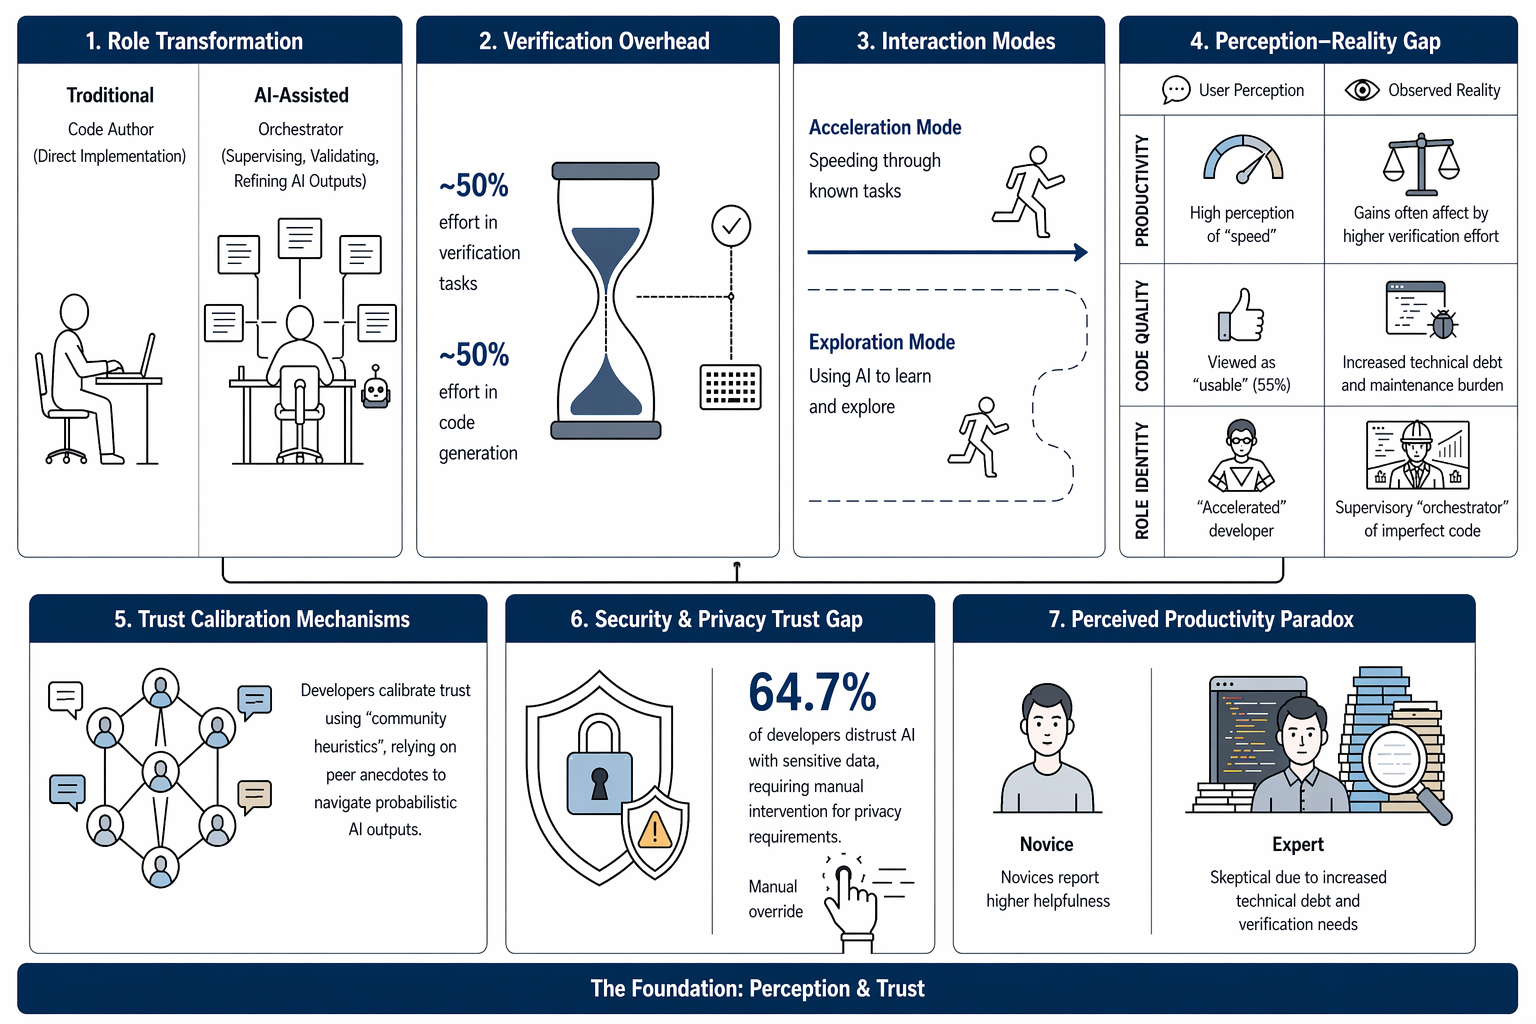
\includegraphics[width=\textwidth]{figures/socio_technical_blueprint.png}
\caption{
Socio-technical blueprint of AI-assisted programming. The figure synthesizes the main findings of this study, illustrating how AI tools reshape development work through effort redistribution, verification overhead, perception–reality gaps, trust calibration mechanisms, and evolving developer roles toward supervision and orchestration.
}
\label{fig:socio-technical-blueprint}
\end{figure*}

Productivity gains are primarily observed in routine and well-defined tasks, while limitations emerge in complex, context-dependent scenarios. These gains are frequently offset by increased effort in validation, coordination, and integration. Across studies, quantitative evidence consistently reinforces that AI-assisted programming delivers measurable gains in output, but these gains are systematically accompanied by trade-offs in reliability, validation effort, and coordination overhead.

At the same time, multiple dimensions—including interaction quality, cognitive load, organisational structure, and trust—act as mediating factors that influence the overall effectiveness of AI-assisted development.

Across studies, these findings suggest that AI-assisted programming is best understood as a socio-technical system, where outcomes are shaped by the interaction between technical capabilities and human, organisational, and contextual factors.

This synthesis suggests that AI-assisted programming is best understood not as a linear improvement in productivity, but as a reconfiguration of development effort across socio-technical dimensions. Its impact emerges from the interaction between technical capabilities and human, organisational, and contextual factors, rather than from any single dimension in isolation.

Taken together, these patterns suggest the emergence of a coherent socio-technical structure underlying AI-assisted programming. These findings are synthesised into a conceptual socio-technical model (Fig.~\ref{fig:socio-technical-blueprint}), which integrates key empirically grounded dynamics identified across the analysis, including effort redistribution, verification overhead, interaction modes, perception–reality gaps, trust calibration mechanisms, and security-related trust gaps. The model captures how these interrelated factors collectively drive a shift in developer roles toward supervision and orchestration, rather than direct code production.

This model should be interpreted as an analytical abstraction derived from observed empirical regularities, rather than as a prescriptive framework, providing a structured lens for understanding the interaction between technical capabilities and socio-technical dynamics.

\section{Discussion}

The socio-technical model presented in Fig.~\ref{fig:socio-technical-blueprint} serves as the central analytical lens and theoretical backbone through which the findings of this study are interpreted.

\subsection{The Productivity Paradox: Faster Development, Uncertain Outcomes}

The results reveal a consistent but nuanced pattern: AI-assisted programming increases development speed, but it does not yet guarantee improved software quality or reliability. High-rigour studies consistently report gains in productivity \cite{cui_productivity_2024, xu_ai-assisted_2026, kumar_intuition_2025}, particularly in routine and well-defined tasks.

However, these gains are often accompanied by increased verification effort, higher rework rates, and potential degradation in code quality \cite{sandoval_lost_2022, zhong_developer-llm_2025}. This tension suggests the presence of a productivity paradox, where increased output does not directly translate into improved outcomes.

Rather than reducing effort, AI-assisted programming redistributes it, shifting developer activity from code generation to validation, debugging, and integration. This finding challenges simplistic narratives of automation and highlights the need to evaluate productivity in terms of total development effort rather than initial output speed.

This shift in effort helps explain the productivity paradox observed across the studies. Empirical evidence shows that time savings in code generation are frequently offset by increased effort in validation and correction \cite{cotroneo_automating_2024, fakhoury_llm-based_2024, eibl_exploring_2025}.

These findings reveal a fundamental distinction between nominal productivity (measured as output volume) and effective productivity (measured as validated, maintainable code). While AI-assisted programming consistently increases the former, it introduces trade-offs that may limit or even reduce the latter.

This shift is particularly evident in team environments, where gains in output from less experienced developers create additional review burdens for more experienced contributors \cite{xu_ai-assisted_2026, koripalli_copilot_2025, kumar_intuition_2025}. As a result, productivity improvements at the individual level do not necessarily translate into net gains at the team level \cite{xu_ai-assisted_2026}.

Moreover, the discrepancy between performance in controlled tasks and real-world development highlights the importance of contextual complexity. While AI tools excel in isolated problem-solving scenarios, their effectiveness declines when tasks require integration, system-level reasoning, or deep domain knowledge \cite{corso_generating_2024, pandey_transforming_nodate, wang_rocks_2024, eibl_exploring_2025}.

These findings suggest that productivity gains should be understood not as absolute improvements but as context-dependent transformations in how development effort is distributed \cite{koripalli_copilot_2025, xu_ai-assisted_2026}.

Overall, the results indicate that AI-assisted programming does not eliminate development effort but transforms its structure, shifting the bottleneck from code production to code validation.

This suggests that AI-assisted programming does not reduce development complexity, but redistributes it across different layers of the socio-technical system.

This paradox can be interpreted as a socio-technical equilibrium, where gains in generation efficiency are systematically balanced by increases in validation, coordination, and cognitive overhead.

Within the socio-technical model, this paradox reflects a structural equilibrium between generation efficiency and verification overhead.

This equilibrium is further shaped by interaction quality and trust calibration, which determine how effectively verification effort translates into reliable outcomes. As a result, productivity should be interpreted as an emergent property of the system rather than as a direct consequence of generation speed alone.

\subsection{The Dominant Role of Human and Contextual Factors}

A key finding across the corpus is that the effectiveness of AI-assisted programming is not determined solely by model capabilities but by human and contextual factors. Interaction quality, prompting strategies, and developer expertise significantly influence outcomes \cite{zhong_developer-llm_2025, pinto_developer_2024}.

In particular, experienced developers appear better equipped to leverage AI tools effectively, while less experienced users may benefit from increased output but struggle with validation and error detection \cite{koripalli_copilot_2025}. This suggests that AI tools amplify existing skill differences rather than eliminating them. An additional emerging concern is the potential impact on long-term skill development. In particular, sustained reliance on AI-assisted tools may reduce engagement with first-principles problem solving among less experienced developers, raising questions about the evolution of human capital in software engineering.

Furthermore, contextual factors such as task complexity, domain specificity, and organisational practices play a critical role. The same tool may produce markedly different outcomes depending on how and where it is used, reinforcing the importance of situational awareness in evaluating AI-assisted development.

These cognitive shifts suggest that the impact of AI-assisted programming extends beyond task performance to fundamental changes in how developers think and work. While AI tools can reduce cognitive load in routine contexts, they simultaneously introduce new cognitive demands related to supervision, validation, and decision-making \cite{tang_study_2024}.

This transformation reflects a shift from generative cognition to evaluative cognition, where the primary challenge is no longer constructing solutions, but assessing their correctness and applicability \cite{tang_study_2024, gardella_performance_2024}.

Put differently, the decisive factor is often not the model itself, but the context in which the model is embedded.

Within the socio-technical equilibrium perspective, these factors act as configuration variables that determine how the balance between generation efficiency and verification effort is achieved. Consequently, system performance depends on the alignment between human capabilities, interaction strategies, and contextual constraints rather than on model performance in isolation.

\subsection{Prompting and Validation as Emerging Meta-Competencies}

The results indicate that effective use of AI-assisted programming requires new forms of expertise beyond traditional coding skills. Prompt formulation, output evaluation, and iterative refinement emerge as critical competencies \cite{pinto_developer_2024, zhong_developer-llm_2025}.

Importantly, interaction with AI systems follows an iterative and adaptive process rather than a single-step query-response pattern. Developers continuously refine prompts, evaluate outputs, and provide corrective feedback, forming a dynamic co-development loop \cite{fayed_prompt-driven_2026, rahe_how_2025, khan_assessing_2023, pinto_developer_2024}.

This interaction model reinforces the view of AI systems as incomplete collaborators, whose effectiveness depends on human guidance rather than autonomous reasoning \cite{borg_echoes_2026, mendes_youre_2024}. The need to structure prompts, detect errors, and contextualise outputs places significant responsibility on the user \cite{bento_leveraging_2025}.

Moreover, the sensitivity of these systems to prompt formulation highlights the emergence of prompting as a design activity \cite{shirafuji_exploring_2023, denny_conversing_2023}. Small variations in input can produce substantially different outputs, requiring developers to think strategically about how problems are framed and communicated to the model \cite{chen_nlperturbator_2026, mastropaolo_robustness_2023}.

In this sense, software development shifts from writing code to orchestrating interactions with generative systems \cite{larbi_when_2025, fayed_prompt-driven_2026}.

This suggests that prompting is not merely an interface mechanism, but a core component of the development process in AI-assisted environments.

The emergence of prompting and validation as core competencies is closely linked to these cognitive changes. As developers rely more on AI-generated outputs, their cognitive effort is increasingly directed toward framing problems, interpreting responses, and detecting inconsistencies \cite{tang_study_2024, gardella_performance_2024}.

This suggests that effective interaction with AI systems requires not only technical knowledge, but also the ability to manage cognitive resources across iterative and uncertain workflows.

In this sense, the primary cognitive challenge in AI-assisted programming shifts from solving problems to evaluating solutions.

This shift suggests a transition in the role of developers, from primary code producers to supervisors of generative systems.

Developers must formulate precise prompts, evaluate outputs, detect subtle errors, and decide when to accept or reject AI-generated suggestions.

These skills, collectively referred to as \textit{prompting and validation literacy}, represent a new layer of professional competence that is essential for effective AI-assisted development.

Within the socio-technical equilibrium model, these competencies directly influence interaction quality and trust calibration, acting as key mechanisms that regulate the balance between generation efficiency and verification overhead. Consequently, differences in prompting and validation literacy explain a significant portion of the variability observed in development outcomes across studies.

\subsection{Reconfiguration of the Developer Role}

The evidence does not support a narrative of developer replacement, but rather one of role transformation. AI-assisted programming shifts the developer's responsibilities from direct implementation toward evaluation, integration, and decision-making \cite{koripalli_copilot_2025, kumar_intuition_2025}.

This reconfiguration aligns with a model of augmented development, where human and AI capabilities are combined rather than substituted. Developers become orchestrators of the development process, managing interactions with AI systems and ensuring the quality and coherence of the final product.

At the same time, this shift raises concerns about potential deskilling, particularly if developers become overly reliant on AI-generated solutions without fully understanding the underlying logic.

Within the socio-technical equilibrium perspective, this role transformation can be understood as a structural consequence of effort redistribution. As generation efficiency increases, direct coding effort is displaced, leading to a corresponding rise in activities related to supervision, validation, and integration. In this sense, the evolution toward an orchestrator role reflects the system's need to maintain balance between generation and verification processes. Consequently, developer effectiveness becomes increasingly dependent on the ability to manage trade-offs across these dimensions rather than on code production alone.

\subsection{Security, Risk, and the Need for Governance}

The findings highlight that AI-assisted programming introduces non-trivial risks, particularly in terms of security and code reliability. Studies report the presence of vulnerabilities, insecure patterns, and logical errors in AI-generated code \cite{sandoval_lost_2022}.

Importantly, these risks are not limited to isolated defects but reflect systematic patterns in AI-generated code. The tendency to produce syntactically correct but semantically shallow solutions, combined with the frequent introduction of security vulnerabilities, suggests that current AI systems systematically optimise for plausibility rather than correctness \cite{sabra_assessing_2025, cotroneo_human-written_2025}.

Moreover, the persistence and amplification of errors across multi-turn interactions indicate that technical debt can accumulate not only from individual outputs but also from the interaction process itself \cite{zhong_developer-llm_2025}. This shifts the locus of risk from static code artefacts to dynamic human--AI interaction processes.

These findings reinforce the need to treat AI-assisted programming as a high-risk augmentation layer, where increased productivity must be balanced with rigorous validation, security practices, and organisational governance \cite{dora_hidden_2025}.

In this sense, AI-assisted programming may function as a systematic catalyst for technical debt, where short-term productivity gains are achieved at the expense of long-term code quality and maintainability.

These risks are compounded by the possibility of over-trust, where developers accept AI-generated outputs without sufficient validation \cite{lyu_my_2025}. Conversely, under-trust may lead to underutilisation of potentially beneficial tools.

This dual risk underscores the need for governance mechanisms, including code review practices, validation pipelines, and organisational policies for AI usage. AI-assisted development should be treated as a socio-technical system requiring structured oversight rather than as a purely technical enhancement.

In practice, this means that the value of AI-assisted programming depends as much on governance quality as on model quality.

This challenge is closely linked to the discrepancy between perceived and actual productivity observed in the results. While developers often report positive experiences with AI tools, the additional effort required for validation and coordination introduces hidden costs that are not always immediately visible \cite{vaillant_developers_2024}.

As a result, trust calibration becomes a critical competency. Developers must learn not only to use AI tools effectively, but also to critically assess their outputs, balancing efficiency with reliability \cite{hicks_new_2024}.

In this context, trust is not a static attribute but a dynamic process shaped by experience, feedback, and organisational practices. Miscalibrated trust—either excessive or insufficient—can significantly impact both individual performance and system-level outcomes \cite{kuhail_will_2024, hicks_new_2024}.

From a socio-technical equilibrium perspective, these risks can be understood as emergent properties of the system, arising from imbalances between generation efficiency, verification capacity, and trust calibration. Governance mechanisms therefore function as stabilising forces that help maintain system equilibrium by constraining error propagation and ensuring that increased output does not compromise reliability.

\subsection{Organisational and Socio-Technical Implications}

Beyond individual productivity, AI-assisted programming has broader organisational implications. The redistribution of tasks within teams, changes in collaboration patterns, and differences in adoption rates all influence outcomes \cite{koripalli_copilot_2025}.

Importantly, the adoption of AI-assisted programming tools leads to a reconfiguration of organisational roles. Developers increasingly transition from direct implementation to supervisory and orchestration functions, managing the interaction between human intent and AI-generated outputs \cite{chen_code_2025}.

This shift introduces new dependencies within teams, where productivity gains at the individual level may create additional coordination and validation burdens at the collective level \cite{weisz_examining_2025}.

The results suggest that successful adoption depends on factors such as training, cultural acceptance, and integration into existing workflows. Organisations that treat AI tools as isolated productivity enhancers may fail to realise their full potential.

Moreover, adoption is not merely a matter of tool availability, but of workflow transformation. Teams that integrate AI tools into their daily practices, communication structures, and task allocation strategies achieve more consistent benefits  \cite{chen_code_2025}.

This suggests that AI-assisted programming is better conceptualised as part of a broader socio-technical system, where technical capabilities interact with human, organisational, and cultural factors \cite{vasiliniuc_case_2023}.

The transition from assistant-based tools to autonomous agent systems further reinforces this socio-technical transformation. While increased autonomy enables more complex task execution, it also introduces new layers of coordination, planning, and risk management \cite{liu_e2edev_2026, yin_comprehensive_2025}.

Rather than simplifying development, agent-based systems shift complexity toward orchestration and control, requiring developers to manage multi-step workflows, monitor system behaviour, and mitigate error propagation \cite{gong_how_2025, he_speed_2026}. This suggests that higher levels of automation do not eliminate human involvement, but instead increase the importance of supervision, governance, and accountability within development processes \cite{gong_how_2025, he_speed_2026}.

In this sense, the impact of AI-assisted programming is mediated not only by individual skill, but by organisational structure and coordination \cite{lyu_will_2025}.

Within the socio-technical equilibrium model, organisations act as higher-level coordination structures that shape how effort redistribution occurs across teams. Effective organisational practices can reduce imbalance between generation and validation activities, while poorly aligned workflows may amplify coordination overhead and degrade overall system performance.

\subsection{Economic Implications and Evidence Gaps}

The analysis reveals that the economic impact of AI-assisted programming cannot be reduced to simple productivity gains. While some studies report positive return on investment under specific conditions, these benefits are counterbalanced by high hidden costs, including supervision, coordination, and interaction overhead \cite{rodriguez_comparative_nodate, song_impact_2024, yin_comprehensive_2025}.

This suggests that economic outcomes should be evaluated in terms of total system cost rather than isolated efficiency improvements. In particular, the emergence of additional cost dimensions—such as prompt formulation effort, validation activities, and computational expenses—highlights the complexity of economic assessment in AI-assisted development environments \cite{nam_understanding_2025, nascimento_comparing_2023}.

Moreover, economic impact appears to be highly context-dependent. Factors such as team structure, developer experience, and workload intensity play a critical role in determining whether AI adoption results in net gains or increased costs \cite{rodriguez_comparative_nodate, song_impact_2024}.

Despite these insights, robust empirical evidence remains limited. This lack of large-scale and longitudinal studies restricts the generalisability of current findings and underscores the need for more comprehensive economic evaluations.

This gap represents an important opportunity for future research, particularly in the form of longitudinal, organisation-level, and cost-aware studies that capture the full complexity of AI-assisted software development.

Within the socio-technical equilibrium perspective, these economic outcomes can be understood as emergent properties of the system, reflecting the balance between gains in generation efficiency and the costs associated with validation, coordination, and interaction. In this sense, economic viability is not determined solely by increased output, but by how effectively organisations manage these trade-offs across the socio-technical system.

\subsection{From Tools to Systems: Increasing Autonomy and Complexity}

The transition from code assistants to more autonomous agent-based systems represents a fundamental shift in software development. While increased autonomy enables more complex task execution, it also introduces additional layers of coordination, planning, and risk management \cite{zhong_developer-llm_2025}.

Rather than simplifying development, higher levels of automation shift complexity toward orchestration, supervision, and control. Developers must manage multi-step workflows, monitor system behaviour, and mitigate error propagation across interconnected processes.

This evolution suggests that AI-assisted programming is not a linear progression toward automation, but a transformation in how development work is structured, governed, and evaluated.

From a socio-technical equilibrium perspective, increasing autonomy amplifies the need for coordination, validation, and control, thereby shifting the system toward higher levels of organisational and cognitive complexity. Rather than eliminating human involvement, autonomous systems redefine it, reinforcing the role of developers as orchestrators responsible for maintaining balance across interconnected processes.

Taken together, the findings suggest that AI-assisted programming is best understood not as a linear improvement in productivity, but as a socio-technical system governed by dynamic trade-offs. The proposed equilibrium perspective provides a unifying explanation for the diverse and sometimes contradictory results reported in the literature, including gains in development speed, increases in verification effort, variability in outcomes, and emerging risks related to quality and security. Under this view, effective adoption depends on the ability to manage these trade-offs across multiple dimensions, including human skills, interaction strategies, and organisational practices.

\section{Theoretical Contributions}

The socio-technical model presented in Fig.~\ref{fig:socio-technical-blueprint} provides the structural foundation for the following theoretical contributions. Together, these contributions articulate complementary aspects of the same underlying system, including its conditional nature, internal equilibrium dynamics, interaction mechanisms, and organisational implications. Each contribution captures a distinct layer of abstraction within this broader socio-technical perspective.

This study makes the following theoretical contributions to the field of software engineering:

\subsection{A Model of Conditional Utility in AI-Assisted Programming}

This study defines the utility of AI-assisted programming as conditional rather than absolute. Its effectiveness depends on the interaction between multiple factors, including task complexity, developer expertise, interaction quality, and level of human supervision.

AI-assisted programming exhibits higher effectiveness in routine and well-defined tasks, with reduced performance in complex, context-dependent scenarios, defining it as a context-sensitive system rather than a universally beneficial tool.

This model challenges deterministic interpretations of AI-assisted programming and instead frames its utility as emergent from the interaction between context, user capability, and task characteristics.

In this sense, the model of conditional utility defines the boundary conditions under which AI-assisted programming produces beneficial outcomes, complementing the equilibrium perspective that explains how trade-offs are managed within those conditions.

\subsection{A Socio-Technical Equilibrium Perspective on AI-Assisted Programming}

Building on the empirical synthesis and the conceptual model presented in Fig.~\ref{fig:socio-technical-blueprint}, this study advances a socio-technical equilibrium perspective on AI-assisted programming. Rather than interpreting AI tools as mechanisms that uniformly increase productivity, their impact emerges from a dynamic balance between multiple interdependent factors. This perspective serves as the central explanatory mechanism that integrates the diverse empirical findings identified across the review.

At the core of this perspective is the relationship in which improvements in code generation efficiency are systematically accompanied by increases in verification effort, coordination overhead, and cognitive load. This relationship defines a structural redistribution of development effort rather than a net reduction in complexity. In this sense, AI-assisted programming operates as a system in which gains in one dimension are offset by trade-offs in others.

The equilibrium perspective is grounded in several empirically observed constructs. First, \textit{generation efficiency} captures the ability of AI tools to accelerate code production. Second, \textit{verification overhead} reflects the additional effort required to validate, correct, and integrate AI-generated outputs. Third, \textit{interaction quality} represents the effectiveness of human--AI communication, particularly through prompting and iterative refinement. Fourth, \textit{trust calibration} captures the extent to which developers appropriately balance reliance on AI outputs with critical evaluation. Finally, \textit{cognitive redistribution} describes the shift in mental effort from code construction toward supervision, validation, and decision-making activities.

These constructs are not independent. Instead, they interact to form a system-level equilibrium. For instance, increases in generation efficiency tend to amplify verification overhead, while higher interaction quality can mitigate this effect by improving output relevance. Similarly, trust calibration acts as a regulating mechanism that determines how much effort is allocated to validation versus acceptance of AI-generated code. As a result, system performance is not determined by any single factor, but by the balance among them.

This perspective reframes AI-assisted programming beyond deterministic productivity interpretations that frame AI-assisted programming as a straightforward productivity enhancer. Instead, it suggests that the effectiveness of these tools depends on how well individuals and organisations manage the inherent trade-offs within the socio-technical system. AI-assisted programming is better understood as a configuration problem, where optimal outcomes emerge from aligning tool capabilities, developer skills, and organisational practices.

By formalising these relationships, this work moves beyond descriptive synthesis and contributes a conceptual lens for understanding AI-assisted software development as a trade-off-driven, socio-technical equilibrium system. This perspective provides a foundation for future empirical research, particularly in investigating how different configurations of these constructs influence development outcomes across contexts.

\subsection{A Human--AI Co-Development Framework}

This work proposes a model of co-development in which AI systems act as incomplete collaborators rather than autonomous agents. Effective workflows follow an iterative cycle of prompt formulation, code generation, validation, correction, and integration.

This framework emphasises that human involvement is not optional but central to achieving reliable outcomes. AI systems extend developer capabilities, but they do not replace the need for human judgement and expertise.

Within the equilibrium perspective, this framework describes the operational interaction layer through which developers regulate the balance between generation and verification activities.

\subsection{Prompting and Validation Literacy as Core Competencies}

This work defines a new layer of professional competence required for effective use of AI-assisted programming tools. Developers must be able to formulate precise prompts, evaluate generated outputs, detect errors, and calibrate trust in AI systems.

These skills, collectively referred to as \textit{prompting and validation literacy}, represent a shift from traditional coding toward higher-order cognitive and evaluative tasks.

Within the equilibrium perspective, prompting and validation literacy represents the competency layer that enables developers to regulate interaction quality, verification effort, and trust calibration. This contribution explains how individual capabilities mediate the relationship between AI-generated outputs and reliable development outcomes.

\subsection{A Socio-Technical Model of AI Adoption}

AI-assisted programming is inherently socio-technical. Its effectiveness depends not only on technical performance but also on organisational practices, team dynamics, and cultural factors.

Adoption outcomes are shaped by training, workflow integration, and shared practices, indicating that AI tools must be understood within the broader ecosystem in which they are deployed.

This perspective extends the equilibrium model to the organisational level, highlighting how institutional structures and team practices influence the configuration and stability of the socio-technical system.

\subsection{A Multi-Dimensional Risk Framework}

This work defines a set of interconnected risks associated with AI-assisted programming, including security vulnerabilities, functional errors, technical debt, over-trust, and potential deskilling.

These risks are not independent: they interact across technical and human dimensions. This reinforces the need for structured validation processes and governance mechanisms when integrating AI tools into software development workflows.

These contributions extend existing perspectives in software engineering by formalising AI-assisted programming as a socio-technical system with conditional and context-dependent utility.

Taken together, these contributions define a unified socio-technical framework in which AI-assisted programming is characterised by conditional utility, equilibrium dynamics, and multi-level interaction across human, technical, and organisational dimensions. This framework provides a conceptual foundation for analysing and designing AI-assisted development practices under varying contextual configurations.

\section{Threats to Validity}

This study is subject to several limitations. First, the dataset includes a proportion of preprint studies that may not have undergone full peer review, which could affect the reliability of some findings. However, these studies were evaluated using a structured quality assessment framework to mitigate this risk.

Second, although artificial intelligence tools were used to support literature discovery and screening, all inclusion, exclusion, and classification decisions were manually validated. Nevertheless, the use of AI-assisted processes may introduce subtle biases in study selection.

Third, the heterogeneity of study designs, evaluation metrics, and experimental contexts limits direct comparability across studies. The included literature spans controlled experiments, observational analyses, and qualitative investigations, which vary significantly in scope and rigour.

Fourth, the analysis relies partially on structured coding of titles, abstracts, and available metadata. While this approach enables large-scale synthesis, it may not capture all nuances present in full-text analyses.

Fifth, differences between perceived and measured outcomes introduce an additional layer of complexity. Some studies report subjective improvements that are not fully aligned with objective performance metrics, which may affect the interpretation of aggregated findings.

Despite these limitations, the combination of systematic screening, quality-based classification, and multidimensional analysis provides a robust foundation for synthesising current evidence on AI-assisted programming.

\section{Conclusion}

This study provides a systematic synthesis of empirical evidence on AI-assisted programming, based on the analysis of 128 studies spanning multiple methodological approaches and analytical dimensions.

The findings confirm that AI-assisted programming can significantly improve developer productivity, particularly in routine and well-defined tasks. However, these gains are conditional and often accompanied by trade-offs in code quality, increased verification effort, and shifts in cognitive and organisational dynamics.

Rather than reducing overall effort, AI tools redistribute it, moving developers' focus from code generation to validation, integration, and decision-making. This transformation challenges the notion of AI as a simple automation mechanism and instead positions it as a catalyst for redefining software development practices.

The study also highlights the importance of human and contextual factors, including developer expertise, interaction quality, and organisational integration. These factors play a decisive role in determining the effectiveness of AI-assisted programming, suggesting that its impact cannot be understood in purely technical terms.

In addition, the analysis identifies significant gaps in the current literature, particularly in the areas of economic evaluation, cognitive impact, and long-term organisational effects. These gaps point to important directions for future research, including longitudinal studies, large-scale economic analyses, and deeper investigation of human--AI collaboration dynamics.

For practitioners, these findings suggest the importance of integrating AI tools within structured validation workflows, investing in developer training for effective prompting, and adopting governance mechanisms to mitigate risks associated with AI-generated code.

Overall, this work contributes to the emerging understanding of AI-assisted programming as a socio-technical phenomenon. Its successful integration requires not only advances in model capabilities but also the development of new skills, practices, and governance structures.

Future research should focus on bridging the gap between short-term productivity gains and long-term software quality, while also exploring longitudinal effects, skill evolution, and the optimisation of human--AI collaboration in real-world environments.

These findings suggest that the future of software development is not defined by automation replacing human effort, but by the emergence of hybrid systems in which human and AI capabilities are tightly coupled. This reinforces the interpretation of AI-assisted programming as a socio-technical equilibrium system rather than a purely productivity-enhancing tool.

Ultimately, the findings indicate that AI-assisted programming delivers value not through linear automation, but through the effective management of interdependent socio-technical factors.

\bibliographystyle{IEEEtran}
\bibliography{references}

\end{document}
